% =======================================================================================
% Chapter 4 -- Results and Discussion
% SECTION-H(13): results presented and discussed in direct correspondence with Chapter 3.
%
% Every number in this chapter is produced by thesis/scripts/thesis_numbers.py from the
% committed result files; none is typed by hand. See Appendix C for the commands.
% =======================================================================================
\chapter{Results and Discussion}
\label{ch:results}

This chapter reports the four experiments of Section~\ref{sec:design} in the order they were
described, followed by the dubbing application, a methodological finding about the measurement
itself, and an overall discussion. All system results are computed on the held-out test split, in
both directions, over 870 attempted utterances.

\section{Corpus Preparation and the Quality Gate}
\label{sec:gate_result}

Feature extraction succeeded on all 2{,}893 linked pairs; no pair was lost to an extraction
error. The quality gate of Section~\ref{sec:corpus_study} then removed 589 pairs, and restriction
to single-speaker pairs removed a further 49, leaving 2{,}304 pairs for the corpus study --- a
drop rate of 20.4\,\%. Table~\ref{tab:gate} lists what each criterion removed. The criteria overlap,
so the individual counts sum to more than the total.

\begin{table}[htbp]
\caption{Pairs removed by each quality criterion, counted if either the English or the Spanish side
failed. Criteria overlap, so the counts are not additive. All criteria are properties of the
measurement and were applied before any outcome was computed.}
\label{tab:gate}
\centering
{\singlespacing\small
\begin{tabular}{@{}lrl@{}}
\toprule
\textbf{Criterion} & \textbf{Pairs affected} & \textbf{Reason} \\
\midrule
F0 not estimable            & 229 & no voiced frames detected on one side \\
Voiced-frame ratio $<0.30$  & 524 & too little voiced speech to characterise pitch \\
Duration outside 0.4--20\,s & 97  & fragment too short or too long to measure \\
Mean F0 outside 60--400\,Hz & 386 & pitch-tracking failure, not a plausible voice \\
\midrule
Different linked speakers   & 49  & pair not performed by a single speaker \\
\midrule
\textbf{Retained}           & \textbf{2{,}304} & 1{,}634 train / 322 dev / 348 test \\
\bottomrule
\end{tabular}\par}
\end{table}

Eleven retained pairs have a mean F0 within 5\,\% of a plausibility bound. They are reported rather
than removed, because removing observations by how far they sit from an expected value would make
the gate depend on the outcome; the median absolute error is reported alongside the mean throughout
Section~\ref{sec:ridge_result} as the robust statistic.

\section{Pipeline Reliability and Intelligibility}
\label{sec:reliability}

Of 870 attempted utterances, 868 completed and 2 failed, a failure rate of 0.23\,\%. Both failures
occurred at the synthesis stage and share one cause: the reference recording was shorter than the
synthesiser's 0.33\,s minimum. The two source utterances are the backchannels \emph{``Mm-hmm.''} and
\emph{``Yeah.''} This is a genuine limitation of the pipeline on very short conversational turns,
and both rows remain in the results file and in the reported rate.

Table~\ref{tab:pipeline} gives the recognition and intelligibility results. Recognition is markedly
harder on Spanish source audio (corpus WER 0.221) than on English (0.150), which matters later:
Section~\ref{sec:cascade} shows that this difference propagates into translation quality.

\begin{table}[htbp]
\caption{Recognition and intelligibility on the held-out test split. Corpus figures pool all edits
over all reference words; speaker means average within each of the 14 test speakers first, then
across speakers, so that no speaker dominates. Lower is better throughout.}
\label{tab:pipeline}
\centering
{\singlespacing\small
\begin{tabular}{@{}lccc@{}}
\toprule
\textbf{Measure} & \textbf{Corpus} & \textbf{Utterance mean} & \textbf{Speaker mean} \\
\midrule
\multicolumn{4}{@{}l}{\emph{\ento{} (English source, $n=433$)}}\\
Recognition WER            & 0.150 & 0.209 & 0.179 \\
Synthesis intelligibility WER & 0.081 & 0.139 & 0.135 \\[0.3em]
\multicolumn{4}{@{}l}{\emph{\esto{} (Spanish source, $n=435$)}}\\
Recognition WER            & 0.221 & 0.265 & 0.263 \\
Synthesis intelligibility WER & 0.087 & 0.135 & 0.114 \\
\bottomrule
\end{tabular}\par}
\end{table}

The synthesis intelligibility figures are low, meaning the generated audio is easy to re-recognise:
re-transcribing the output and comparing against the text that was sent to the synthesiser gives a
corpus WER of 0.081 and 0.087. Only three of 868 outputs produced an empty re-transcription. The
synthesiser is therefore producing clearly articulated speech; whatever it fails to preserve, it is
not intelligibility.

The gap between the corpus figure and the utterance mean is worth one remark, because it recurs in
every WER row. Corpus WER weights each utterance by its length; the utterance mean weights every
utterance equally, so a single wrong word in a three-word backchannel counts as heavily as ten
errors in a thirty-word turn. A conversational corpus is full of short turns, so the mean is always
the higher figure. Both are reported because they answer different questions, and neither is
presented alone.

\section{Translation Quality and Cascade Error Propagation}
\label{sec:cascade}

Corpus BLEU on the full cascade is 22.14 for \ento{} and 23.45 for \esto{}, with chrF at 47.22 and
46.63 respectively. These absolute values must be read with the caution of
Section~\ref{sec:instruments}: the reference is a spoken \emph{re-enactment}, so it is a legitimate
rendition of the same content but not a sentence-level gloss, and the scores are correspondingly
lower than the same models achieve on written parallel text. Differences against the same reference
remain interpretable.

The fine-tuning experiment supplies a second measurement of the same models translating the
\emph{human} transcript rather than the recogniser output, on the same test utterances and under
identical decoding. The difference between the two isolates the cost of the recognition stage
(Figure~\ref{fig:cascade}).

\begin{figure}[htbp]
\centering
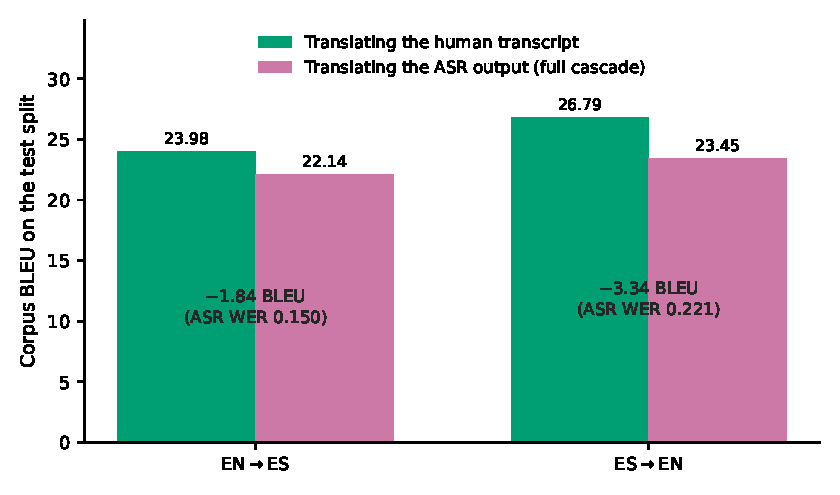
\includegraphics[width=0.78\linewidth]{figures/F_cascade_error.pdf}
\caption{Cost of automatic recognition in the cascade. The same translation model, the same test
utterances and identical decoding; the only difference is whether the input is the human transcript
or the Whisper output. The loss is larger in the direction where recognition is worse.}
\label{fig:cascade}
\end{figure}

Recognition errors cost 1.84 BLEU in \ento{} and 3.34 BLEU in \esto{}. The ordering is the
important part: the larger loss occurs in the direction with the higher recognition error rate
(0.221 against 0.150). This is the classic weakness of cascaded speech translation
\cite{sperber2020endtoend}, measured here on the project's own data rather than cited, and it is a
quantitative argument for the end-to-end approaches reviewed in Section~\ref{sec:lit_s2st}. It also
identifies where effort would pay: on Spanish source audio, an improvement in recognition is worth
roughly twice as much downstream as the same improvement on English.

\section{Speaker Identity Against the Human Ceiling}
\label{sec:identity_result}

Speaker similarity between the source recording and the synthesised output is 0.421 for \ento{}
and 0.383 for \esto{} (speaker means). In isolation these numbers are uninterpretable. The
same-speaker design supplies the missing scale: the same speaker's real recording in the other
language scores 0.445 in both directions. Against that ceiling the system retains \textbf{94.5\,\%}
and \textbf{86.1\,\%} of the achievable similarity (Figure~\ref{fig:identity}).

\begin{figure}[htbp]
\centering
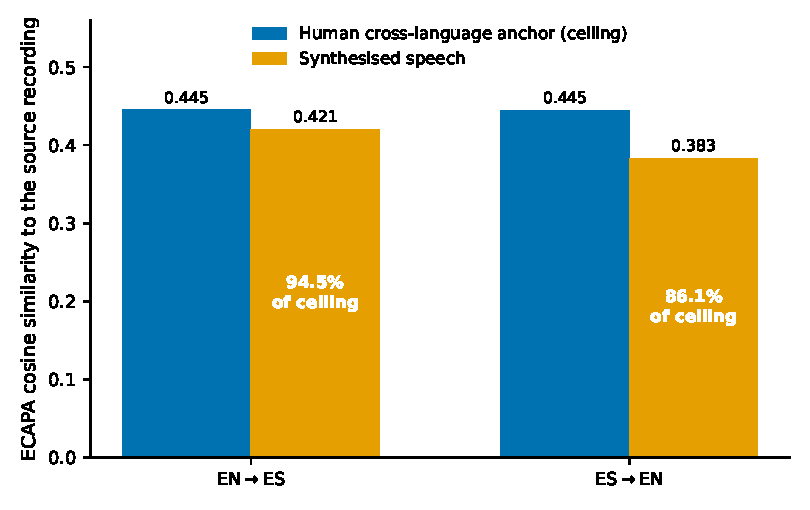
\includegraphics[width=0.72\linewidth]{figures/F_identity_ceiling.pdf}
\caption{Speaker identity measured against the human cross-language ceiling. The ceiling is the
ECAPA cosine between the source recording and the \emph{same speaker's} real recording in the other
language; it is available only because the corpus is same-speaker parallel.}
\label{fig:identity}
\end{figure}

Three observations follow.

First, the ceiling itself is low --- 0.445, not 0.9. Two genuine recordings of one person, in two
languages, are only that similar under an ECAPA cosine. Any evaluation that reports a raw cosine
of 0.42 as poor preservation is applying a standard that human speech does not meet either.

Second, the two ceilings are near-identical (0.4452 and 0.4450), as they must be, since both
compare the same pair of human recordings with the roles exchanged. The asymmetry between 94.5\,\%
and 86.1\,\% is therefore entirely in the synthesiser's output: cloning works better \emph{into}
Spanish than into English. A plausible explanation is the language balance of the synthesiser's
training data, but that was not tested here and is offered as a hypothesis, not a finding.

Third, the aggregate conceals real variation. Per speaker, the percentage of ceiling ranges from
74.7\,\% to 147.2\,\% in \ento{} (median 90.7\,\%) and from 55.5\,\% to 107.9\,\% in \esto{}
(median 85.8\,\%). Values above 100\,\% occur where the synthesised output resembles the source
recording more closely than the speaker's own other-language recording does --- which is possible,
because the synthesised audio inherits channel and recording characteristics from the reference
clip that the human's second recording need not share. The test split is also unbalanced, ranging
from 2 to 118 pairs per speaker, which is why every aggregate in this chapter is a speaker mean
rather than a mean over rows.

\section{Cross-Lingual Prosody in Human Speech}
\label{sec:corpus_result}

Before the system can be judged, the human behaviour it is being compared against must be
established. Table~\ref{tab:corpusprosody} characterises how the same speaker's prosody differs
between their English and Spanish renditions of the same content, over 2{,}304 pairs from 94
speakers, 92 of whom contribute more than one pair and therefore enter the within-speaker
decomposition.

\begin{table}[htbp]
\caption{Cross-lingual prosody of the same speaker over 2{,}304 same-speaker pairs. $\Delta$ is the
paired mean difference (Spanish minus English) with a 95\,\% confidence interval. F0 is in
semitones relative to 100\,Hz.}
\label{tab:corpusprosody}
\centering
{\singlespacing\small
\begin{tabular}{@{}lrrrrr@{}}
\toprule
\textbf{Measure} & \textbf{English} & \textbf{Spanish} & \textbf{$\Delta$ (ES$-$EN)} &
\textbf{95\,\% CI} & \textbf{Pooled $r$} \\
\midrule
F0 level (st)        & 8.51 & 8.67 & $+0.16$ & $[0.08,\,0.24]$ & 0.952 \\
F0 range (st)        & 2.31 & 2.23 & $-0.08$ & $[-0.16,\,-0.00]$ & 0.263 \\
Duration (s)         & 2.73 & 2.85 & $+0.12$ & $[0.09,\,0.15]$ & 0.870 \\
Speaking rate (w/s)  & 3.42 & 3.07 & $-0.36$ & $[-0.40,\,-0.32]$ & 0.595 \\
\bottomrule
\end{tabular}\par}
\end{table}

The systematic language-level differences are small but statistically clear. Spanish renditions sit
0.16 semitones higher in pitch, run 0.12\,s longer, and are spoken 0.36 words per second slower;
the median Spanish-to-English duration ratio is 1.049 (Figure~\ref{fig:corpusdur}). All four
confidence intervals exclude zero, although Figure~\ref{fig:paireddeltas} shows that each shift is
small relative to the spread of individual pairs.
For the purposes of this study, however, the interesting quantity is not the mean shift but the
\emph{correspondence}: how strongly one speaker's English behaviour predicts their own Spanish
behaviour. Figure~\ref{fig:corpusf0} shows this for pitch.

\begin{figure}[htbp]
\centering
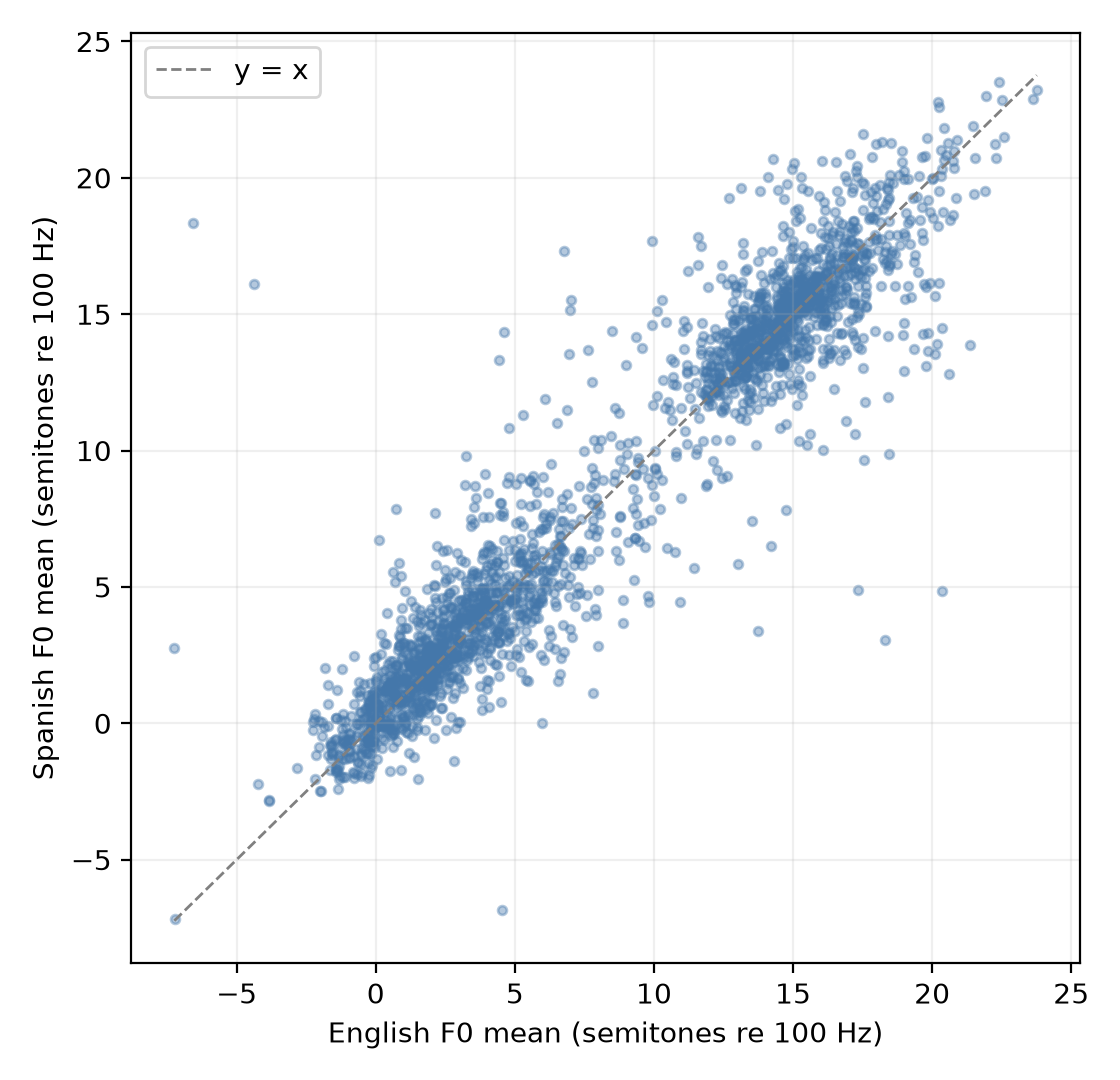
\includegraphics[width=0.72\linewidth]{figures/F_corpus_f0_scatter.png}
\caption{English against Spanish mean F0 in semitones for the same speaker and the same content,
over 2{,}304 pairs. The tight relationship along the diagonal is what makes a human cross-language
prosody ceiling meaningful.}
\label{fig:corpusf0}
\end{figure}

Pooled correlations are high for pitch level (0.952) and duration (0.870), moderate for speaking
rate (0.595) and weak for pitch range (0.263). The pooled figures are not, however, the right
answer, and Section~\ref{sec:prosody_gap} decomposes them.

\section{The Prosody Transfer Gap}
\label{sec:prosody_gap}

This is the central result of the dissertation. Table~\ref{tab:prosodygap} places the system's
prosody, measured against the human target-language recording, beside the human's own
cross-language correspondence for the same features and the same measurement procedure, and
Figure~\ref{fig:prosodygap} plots the within-speaker columns of that table.

\begin{table}[htbp]
\caption{Cross-lingual prosody correspondence, human against system. Every correlation is with the
human target-language recording. \emph{Within-speaker} removes each speaker's own mean before
correlating and is the figure that answers the research question; \emph{pooled} is shown to expose
how much of it is speaker identity rather than prosody transfer.}
\label{tab:prosodygap}
\centering
{\singlespacing\small\setlength{\tabcolsep}{4.5pt}
\begin{tabular}{@{}lcccccc@{}}
\toprule
& \multicolumn{2}{c}{\textbf{Human \enes{}}}
& \multicolumn{2}{c}{\textbf{System \ento{}}}
& \multicolumn{2}{c}{\textbf{System \esto{}}} \\
\cmidrule(lr){2-3}\cmidrule(lr){4-5}\cmidrule(lr){6-7}
\textbf{Measure} & Pooled & Within & Pooled & Within & Pooled & Within \\
\midrule
F0 level      & 0.952 & \textbf{0.849} & 0.698 & \textbf{0.311} & 0.754 & \textbf{0.314} \\
F0 range      & 0.263 & \textbf{0.214} & 0.142 & \textbf{0.035} & 0.132 & \textbf{0.040} \\
Duration      & 0.870 & \textbf{0.867} & 0.364 & \textbf{0.352} & 0.618 & \textbf{0.610} \\
Speaking rate & 0.595 & \textbf{0.601} & 0.360 & \textbf{0.372} & 0.353 & \textbf{0.346} \\
Energy        & ---   & ---            & 0.076 & \textbf{0.090} & 0.057 & \textbf{0.060} \\
\midrule
$n$ (pairs)   & \multicolumn{2}{c}{2{,}304} & \multicolumn{2}{c}{345--433}
              & \multicolumn{2}{c}{374--435} \\
\bottomrule
\end{tabular}\par}
\end{table}

\begin{figure}[htbp]
\centering
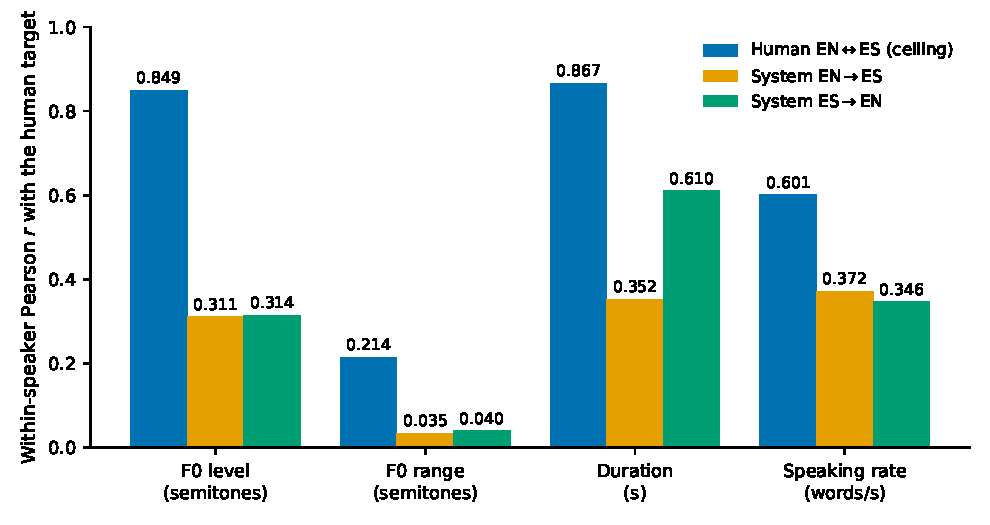
\includegraphics[width=0.92\linewidth]{figures/F_prosody_gap.pdf}
\caption{Within-speaker cross-lingual prosody correspondence. The blue bars are what a human
achieves when re-enacting their own utterance in the other language; the orange and green bars are
what the system achieves against that same human recording.}
\label{fig:prosodygap}
\end{figure}

\textbf{Pitch level.} A human re-enacting their own utterance in the other language reproduces
their pitch level at $r=0.849$ within-speaker. The system reaches $0.311$ and $0.314$ --- about
37\,\% of the human figure. The mechanism is known and was stated in advance
(Section~\ref{sec:lit_tts}): the synthesiser is conditioned on the reference recording for timbre
and is never given the source pitch contour, so it must invent intonation from the target text.

\textbf{Pitch range collapses.} Human within-speaker correspondence for F0 range is already modest
at $0.214$; the system reaches $0.035$ and $0.040$, which is effectively no relationship at all.
Utterance-level expressive variation --- the part of prosody that distinguishes an excited turn
from a flat one --- does not survive the pipeline.

\textbf{Duration survives best.} The system reaches $0.352$ and $0.610$ against a human $0.867$.
This is unsurprising: utterance duration is largely determined by how much there is to say, and the
translated text preserves the content. It is also the feature the dubbing application can repair
by post-processing, which the other features are not.

\textbf{Energy carries essentially nothing} ($0.076$ and $0.057$ pooled), which is expected, since
recording level is a property of the microphone and gain rather than of the speaker.

\subsection{Why the Pooled Figures Must Not Be Quoted Alone}
\label{sec:pooled_warning}

Comparing the pooled and within-speaker columns of Table~\ref{tab:prosodygap} makes the point.
For the system's pitch level, the pooled correlation is $0.698$ and $0.754$, while the
within-speaker correlation is $0.311$ and $0.314$. The between-speaker correlation --- computed
over one point per speaker --- is $0.895$ and $0.847$, and speaker differences account for 47\,\%
and 61\,\% of the total variance in the measurement. Figure~\ref{fig:pooledwithin} shows the
contrast.

\begin{figure}[htbp]
\centering
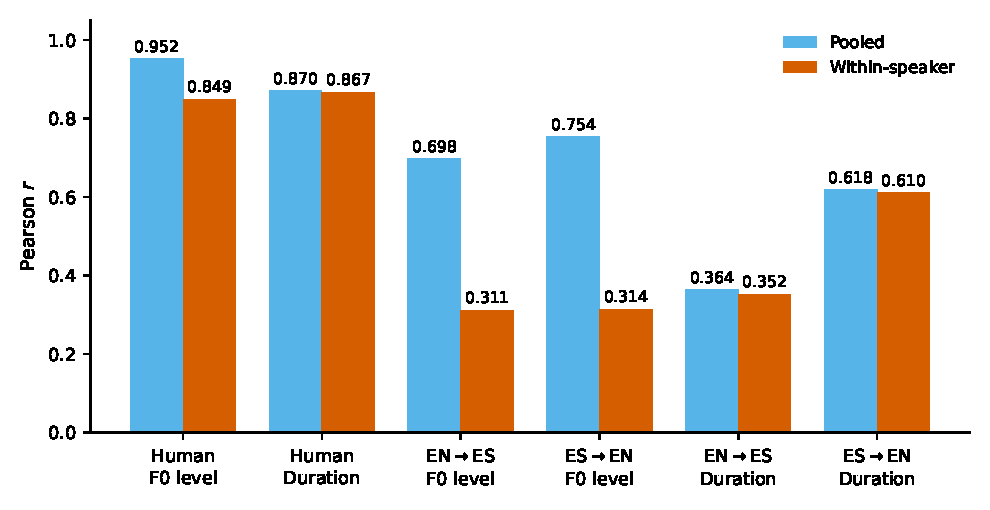
\includegraphics[width=0.92\linewidth]{figures/F_pooled_vs_within.pdf}
\caption{Pooled against within-speaker correlation. Where the two differ sharply, as they do for
the system's pitch level, most of the pooled figure is stable between-speaker variation --- a
low-pitched person remaining low-pitched --- carried by voice cloning rather than by prosody
transfer. Duration, where the two nearly coincide, is a genuine correspondence.}
\label{fig:pooledwithin}
\end{figure}

Read correctly, this is not a weaker version of the result but a sharper one. A pooled correlation
near $0.75$ would ordinarily be reported as strong prosody transfer. It is not. It is the voice
clone reproducing the speaker's habitual pitch --- which is exactly the identity result of
Section~\ref{sec:identity_result} appearing a second time under a different name. Once speaker
identity is removed, what remains is $0.31$: the same pipeline that preserves identity well
preserves utterance-level prosody poorly. Reporting the pooled figure alone would have
attributed the success of one component to another.

\subsection{Relation to the Literature}

This quantifies precisely the gap that expressive dubbing systems exist to close.
\citeA{swiatkowski2023dubbing} developed a cross-lingual prosody representation for machine
dubbing without access to parallel expressive data; \citeA{song2023styles2st} pursued the same goal
inside a direct S2ST model. The contribution here is complementary rather than competing: it is not
a better system but a calibrated statement of the size of the problem, expressed in units --- a
within-speaker correlation against a human ceiling --- that any subsequent system can be measured
in.

\section{Predicting Target-Language Prosody}
\label{sec:ridge_result}

Section~\ref{sec:prosody_gap} shows the system does not transfer prosody. This section asks a
narrower question: is target-language prosody \emph{predictable} from the source at all? If it is
not, no amount of conditioning would help.

Table~\ref{tab:ridge} reports the test-split result for each direction and target, against the
three baselines of Section~\ref{sec:ridge}. Figure~\ref{fig:ridge} shows the same comparison
graphically.

\begin{table}[htbp]
\caption{Prosody prediction on the held-out test split, in mean absolute error (lower is better).
$\Delta$ is the change relative to the copy-plus-offset baseline B2; $p$ is a Wilcoxon signed-rank
test on per-speaker mean absolute errors ($n=14$ speakers), which is the appropriate unit of
independence. F0 targets are in semitones, duration in log-ratio.}
\label{tab:ridge}
\centering
{\singlespacing\small\setlength{\tabcolsep}{4.5pt}
\begin{tabular}{@{}llrrrrrr@{}}
\toprule
\textbf{Direction} & \textbf{Target} & \textbf{B1} & \textbf{B0} & \textbf{B2} &
\textbf{Ridge} & \textbf{$\Delta$ vs B2} & \textbf{$p$} \\
\midrule
\ento{} & F0 level      & 5.783 & 1.375 & 1.353 & \textbf{1.353} & $-0.02\,\%$ & 0.0040 \\
\ento{} & F0 range      & 1.034 & 0.977 & 0.983 & \textbf{0.932} & $-5.14\,\%$ & 0.0012 \\
\ento{} & Duration ratio& 0.181 & 0.186 & 0.181 & \textbf{0.180} & $-0.73\,\%$ & 0.1937 \\
\midrule
\esto{} & F0 level      & 5.947 & 1.350 & 1.329 & \textbf{1.329} & $-0.00\,\%$ & 0.9032 \\
\esto{} & F0 range      & 1.017 & 0.963 & 0.968 & \textbf{0.931} & $-3.89\,\%$ & 0.0001 \\
\esto{} & Duration ratio& 0.182 & 0.187 & 0.182 & \textbf{0.172} & $-5.34\,\%$ & 0.1040 \\
\bottomrule
\end{tabular}\par}
\end{table}

\begin{figure}[htbp]
\centering
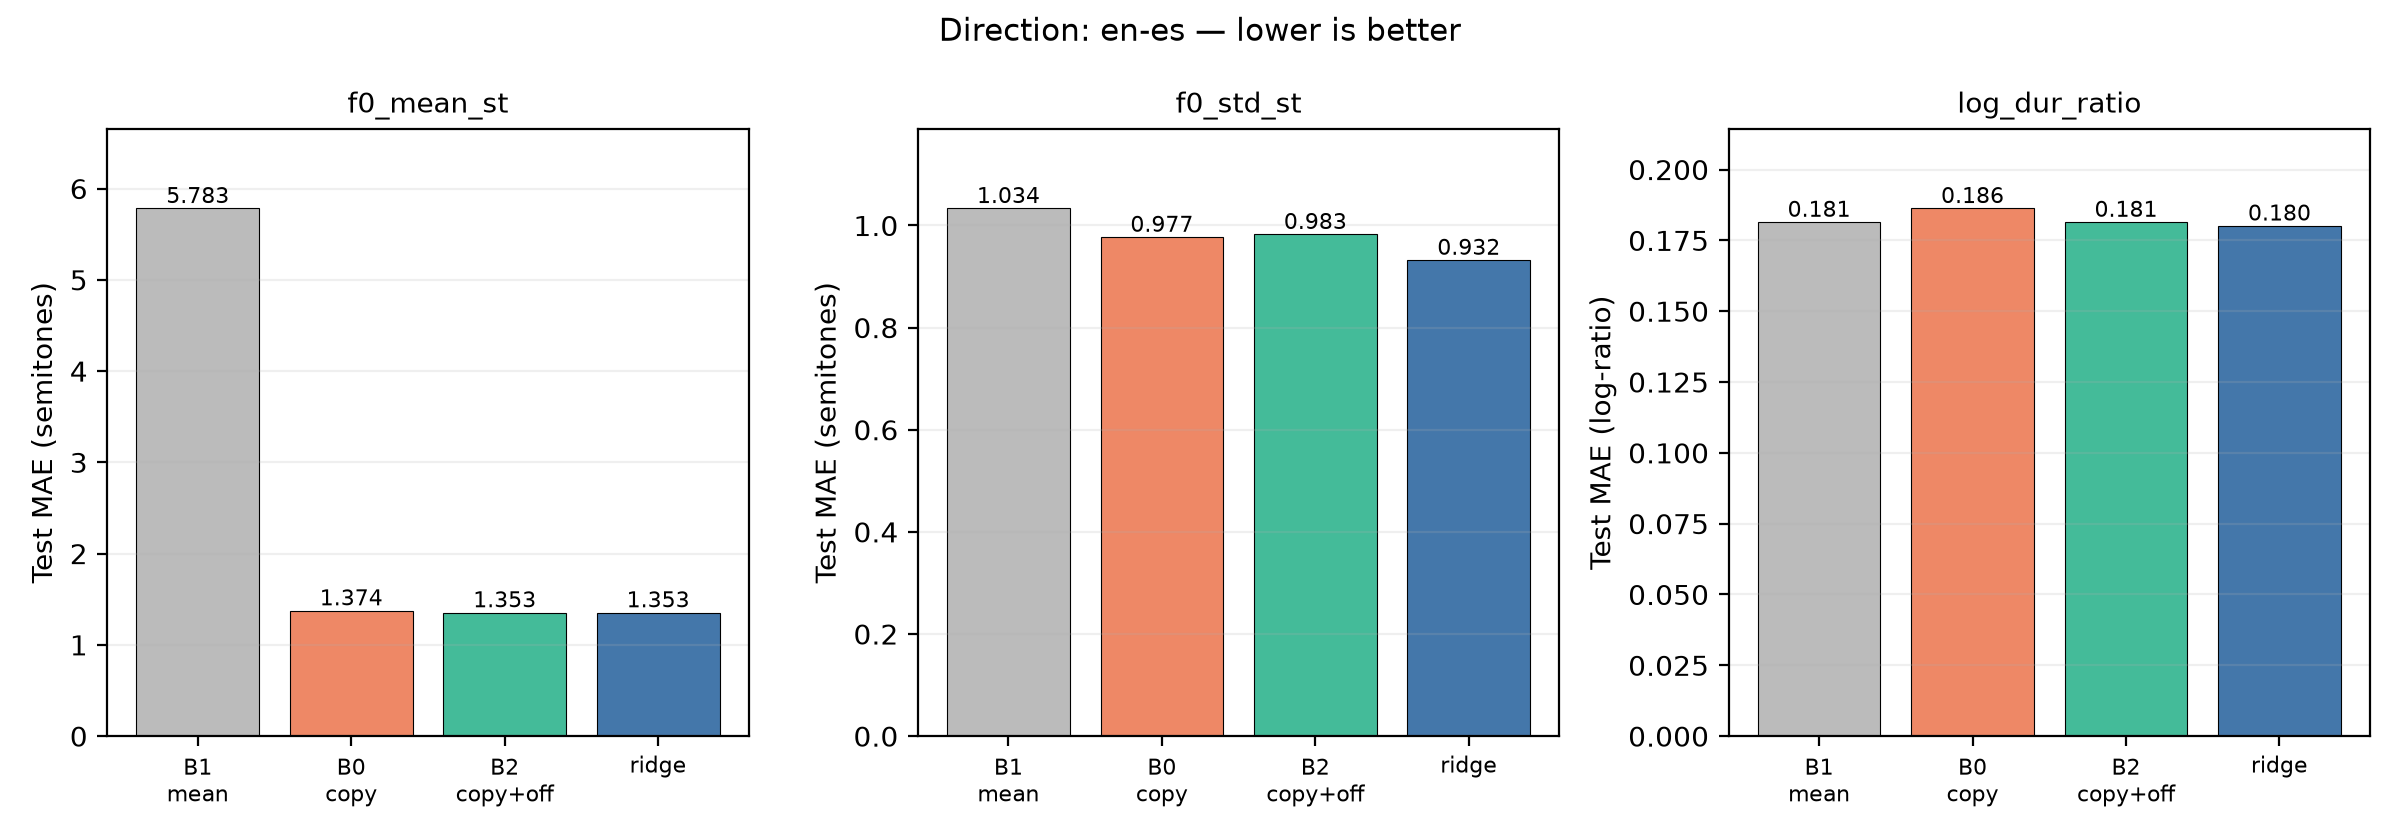
\includegraphics[width=0.86\linewidth]{figures/F_ridge_mae_en-es.png}
\caption{Test mean absolute error for each prosody target in the \ento{} direction, model against
the three baselines. The trivial baseline B1, which ignores the source entirely, is catastrophic
for pitch level; the informative comparison is against B2.}
\label{fig:ridge}
\end{figure}

\subsection{What the Result Says}

\textbf{Pitch level is not predictable beyond the baseline.} The improvement is $-0.02\,\%$ and
$-0.00\,\%$: numerically nothing. The regulariser selected $\lambda=10^{6}$ in both directions, at
which every weight is effectively zero, so the model \emph{chose} to become the baseline. This is
not a failure of fitting but the regulariser reporting honestly that no conditional signal is
available. It is also strong evidence against overfitting.

\textbf{Pitch range is predictable, in both directions.} The model reduces mean absolute error by
$5.14\,\%$ (\ento{}) and $3.89\,\%$ (\esto{}), with speaker-clustered $p$ of 0.0012 and 0.0001 and
bootstrap confidence intervals for the difference that exclude zero; Figure~\ref{fig:ridgeesen} in
Appendix~\ref{app:figures} shows the \esto{} direction. The mechanism is visible in the fitted
coefficients (Table~\ref{tab:coefficients}): the weight on source F0 range is $-0.191$ and
$-0.143$ --- large relative
to the other five weights, and \emph{negative}. The model has learned that an unusually wide
source pitch range should be predicted narrower in the target: per-utterance variation regresses
towards the speaker's typical range rather than transferring one for one. That is an interpretable
finding about cross-lingual prosody, not merely a number.

\textbf{Duration ratio is not reliably predictable.} The nominal improvement of $5.34\,\%$ in
\esto{} does not survive clustering by speaker ($p=0.104$).

\subsection{Multiple Comparisons}
\label{sec:multiplicity}

Six models were fitted, so the family-wise position must be stated rather than left implicit.
Under Bonferroni at $\alpha=0.05$ the threshold is $0.05/6=0.0083$; three of the six
speaker-clustered $p$-values fall below it (0.0001, 0.0012, 0.0040), and the same three survive
Holm and Benjamini--Hochberg at 5\,\%. Only two of those three are practically meaningful: the F0
range results in both directions. The third, \ento{} pitch level, is statistically detectable and
practically nil, an effect of $-0.02\,\%$ that arises because the model is numerically almost
identical to the baseline it is being compared against --- a signed-rank test over near-identical
error vectors can return a small $p$ for a zero-sized effect. It is reported here so that it cannot
be quoted as a third success.

The defensible claim is therefore narrow and consistent: \emph{the predictable component of
cross-lingual prosody lies in pitch range, not in pitch level or timing}, supported by agreement in
sign and magnitude across both directions, by survival of family-wise correction, and by a
coefficient whose value explains the mechanism.

\section{Fine-Tuning the Translation Component}
\label{sec:finetune_result}

Fine-tuning on 1{,}998 in-domain sentence pairs improved reference-matching in both directions,
on a held-out test set of unseen speakers under identical decoding (Figure~\ref{fig:finetune}).
For \ento{}, BLEU rose from 23.98 to 26.31 and chrF from 49.87 to 51.70, a gain of $+2.34$ and
$+1.82$. For \esto{}, BLEU rose from 26.79 to 30.02 and chrF from 50.30 to 52.27, a gain of
$+3.23$ and $+1.97$.

\begin{figure}[htbp]
\centering
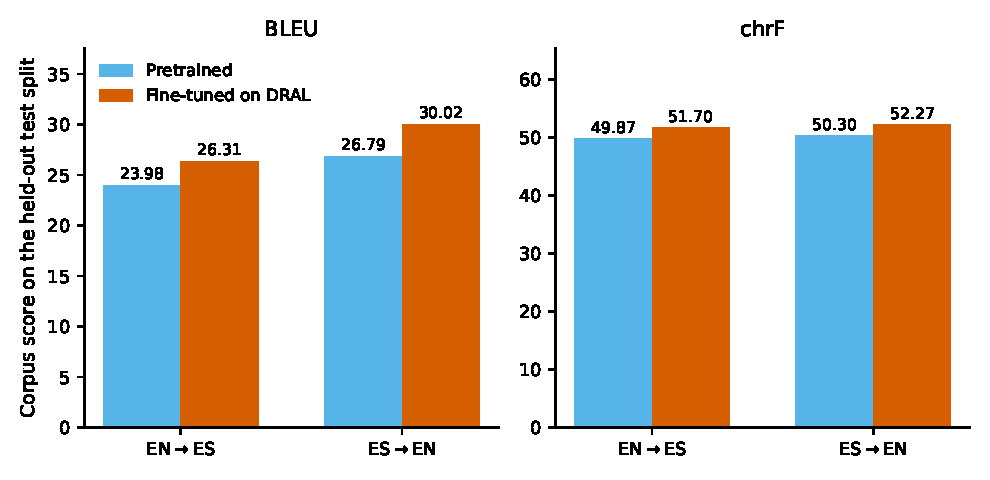
\includegraphics[width=0.92\linewidth]{figures/F_finetune_bleu_chrf.pdf}
\caption{Translation quality before and after in-domain fine-tuning, on the held-out test split
($n=432$ per direction) with identical decoding settings for both systems.}
\label{fig:finetune}
\end{figure}

The checkpoint was selected on development loss, and the selection is the methodologically
important part. Table~\ref{tab:losses} shows textbook overfitting: training loss falls
monotonically while development loss reaches its minimum at epoch 2 and rises thereafter. Both
directions independently selected epoch 2, as Figures~\ref{fig:ftcurveenes}
and~\ref{fig:ftcurveesen} in Appendix~\ref{app:figures} show. The test split was scored once,
after selection.

\begin{table}[htbp]
\caption{Training and development loss per epoch. Development loss is minimised at epoch~2 in both
directions, and the epoch-2 checkpoint was selected on that basis before the test split was
touched.}
\label{tab:losses}
\centering
{\singlespacing\small
\begin{tabular}{@{}ccccc@{}}
\toprule
& \multicolumn{2}{c}{\textbf{\ento{}}} & \multicolumn{2}{c}{\textbf{\esto{}}} \\
\cmidrule(lr){2-3}\cmidrule(lr){4-5}
\textbf{Epoch} & Train & Dev & Train & Dev \\
\midrule
1 & 1.922 & 1.730 & 1.614 & 1.378 \\
2 & 1.569 & \textbf{1.712} & 1.337 & \textbf{1.361} \\
3 & 1.368 & 1.744 & 1.165 & 1.382 \\
4 & 1.221 & 1.790 & 1.032 & 1.432 \\
\bottomrule
\end{tabular}\par}
\end{table}

\begin{caveat}
The BLEU gain is register and style adaptation, not improved translation adequacy. The corpus's
Spanish side is a re-enactment, so matching the reference more closely means sounding more like
these particular speakers, not translating better. In the fine-tuned outputs, \emph{bicicleta}
becomes \emph{bici} and \emph{presa} becomes \emph{represa}; \emph{nos ayudamos mutuamente} becomes
\emph{nos ayudamos el uno al otro}. In several cases the pre-trained output is the better
standalone translation. That chrF moves less than BLEU ($+1.8$ against $+2.3$) is consistent with
this reading, since chrF is character-based and comparatively robust to lexical substitution and
word-order change.
\end{caveat}

\subsection{Why Only the Translation Component Was Adapted}
\label{sec:why_only_mt}

Recognition already achieves a corpus WER of 0.150 on English source audio, leaving little
headroom, and adapting a large recogniser on 1{,}998 utterances of one corpus would risk harming
generalisation. Adapting the synthesiser requires substantially more data and compute than a
laptop provides. Translation is the cheapest experiment with a clear domain mismatch to exploit
and a well-understood metric: 12.4 and 10.8 minutes of training respectively. The choice is an
engineering judgement about where a limited budget buys the most information, and it is stated as
such.

\subsection{Reconciling the Progress-Report BLEU}
\label{sec:bleu61}

The progress report submitted in January 2026 quoted a BLEU of approximately 61, whereas this study
measures the pre-trained model at 23.98. Both figures are correct, and they measure different
things. The earlier figure was a \emph{back-translation} score: the Spanish output was translated
back to English and compared against the original English text. That is a much easier comparison,
because errors introduced on the outward pass can cancel on the return. The figures in this chapter
are computed against an independent human reference. The change is a change of instrument, not a
regression in the system.

\section{Duration Inflation and the Retiming Stage}
\label{sec:duration_result}

Raw synthesised speech is systematically longer than the speech it replaces. Averaged over the test
split, generated utterances run 4.07\,s against a human target of 2.67\,s, a ratio of
$1.52\times$; the median per-utterance ratio is $1.43$, and 25.1\,\% of utterances exceed
$2.0\times$ (Figure~\ref{fig:durationratio}). The inflation is worse in \ento{} (median $1.51$)
than in \esto{} (median $1.32$).

\begin{figure}[htbp]
\centering
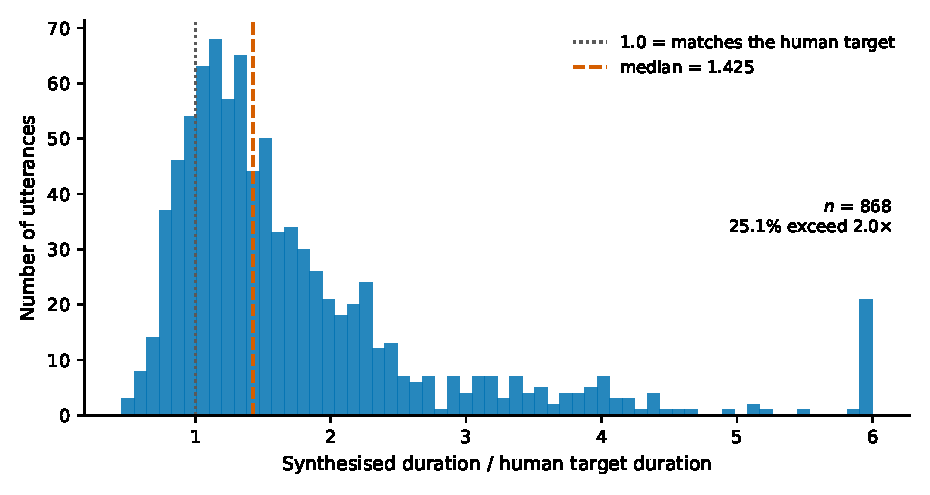
\includegraphics[width=0.82\linewidth]{figures/F_duration_ratio.pdf}
\caption{Ratio of synthesised duration to human target duration over all 868 successful
utterances, clipped at $6\times$ for display. The distribution sits clearly to the right of 1.0:
the inflation is a systematic bias, not random error.}
\label{fig:durationratio}
\end{figure}

This is not a subtle effect and it is fatal for dubbing: at $1.5\times$ per utterance, a dubbed
track drifts out of synchronisation with the picture within a few turns. It is the reason the
application includes the WORLD retiming stage described in Section~\ref{sec:webapp}.

\subsection{Behaviour of the Dubbing Application}
\label{sec:dubbing_result}

Table~\ref{tab:dubbing} reports five real dubbing jobs, 83 segments in total. The retiming stage
works, and its limit is visible.

\begin{table}[htbp]
\caption{Five dubbing jobs. \emph{Raw ratio} is synthesised duration over the original slot before
retiming; \emph{final match} is the dubbed track length over the original after retiming, where
1.000 is perfect. \emph{Clamped} counts segments needing a scale outside the permitted
$0.5\times$--$2.0\times$ range.}
\label{tab:dubbing}
\centering
{\singlespacing\small\setlength{\tabcolsep}{4.5pt}
\begin{tabular}{@{}lcrrrrr@{}}
\toprule
\textbf{Job} & \textbf{Direction} & \textbf{Segments} & \textbf{Clamped} &
\textbf{Raw ratio} & \textbf{Final match} & \textbf{Identity} \\
\midrule
f44255c7 & \esto{} & 3  & 0 (0\,\%)   & 0.785 & \textbf{1.001} & 0.422 \\
dafbca94 & \esto{} & 4  & 1 (25\,\%)  & 1.243 & 1.056 & 0.718 \\
0d472aee & \esto{} & 22 & 5 (23\,\%)  & 1.510 & 1.062 & 0.619 \\
44e83311 & \ento{} & 15 & 1 (7\,\%)   & 1.583 & 1.067 & 0.385 \\
3ae892f4 & \ento{} & 39 & 23 (59\,\%) & 2.173 & 1.226 & 0.260 \\
\bottomrule
\end{tabular}\par}
\end{table}

Where the raw ratio is at or below about $1.6\times$, retiming brings the dubbed track to within
7\,\% of the original length and the clamp binds on at most a quarter of segments. Where the raw
ratio reaches $2.17\times$, the clamp binds on 59\,\% of segments, and the final track is 22.6\,\%
too long. The failure mode is worth stating precisely, because it explains what a listener hears: a
0.84\,s slot receiving 7.61\,s of synthesised speech would need a scale of $0.11\times$; the floor
of $0.5\times$ produces 3.81\,s, which is 2.97\,s too long, and that overflow lands on top of the
following segment. Segments are summed into the timeline, so two voices speak at once.

The diagnosis identifies the correct fix, and it is upstream. No amount of digital signal
processing can absorb a $2.17\times$ length ratio without destroying the audio. The real problem is
that the translation model produces an utterance whose spoken length was never constrained ---
exactly the problem that length-controlled translation for dubbing was designed to solve
\cite{lakew2021verbosity,federico2020dubbing}. This is the first item of future work in
Section~\ref{sec:future}.

Two secondary observations. Speaker identity measured on the retimed output ranges from 0.260 to
0.718 across jobs, and the lowest value is the job with the highest clamp rate, which is
consistent with heavy time-scaling degrading the voice. And the pipeline is slow: roughly
13$\times$ real time on the test machine, because synthesis is inherently sequential and runs on
the CPU.

\section{A Correction to the Measurement Itself}
\label{sec:f0correction}

One finding of this project is about its own instrument, and it is reported because the earlier
conclusion it overturned was wrong by roughly a factor of seven.

An earlier version of the analysis reported that the system transferred essentially no pitch
information: a correlation of $0.090$ between generated and human-target F0. Two defects produced
that number.

\textbf{Correlating pitch in hertz.} Pitch perception is logarithmic, so a correlation computed in
hertz is dominated by whichever values lie furthest from the mean, and a single octave-doubled
observation is enough to destroy it. On identical underlying measurements, correlating in
semitones instead of hertz moved the \ento{} F0 correlation from $0.048$ to $0.368$.

\textbf{No plausibility gate.} The pitch tracker's search band admits occasional octave doublings.
Excluding observations whose median F0 falls outside the plausible adult speaking range --- a
criterion on the measurement, not on the outcome --- moved the same figure from $0.368$ to $0.820$.

A third intervention, attempted first, made matters worse and is recorded because the reasoning
behind it was wrong in an instructive way. Narrowing the pitch tracker's \emph{search} band to
60--400\,Hz seemed the natural remedy for octave errors. Measured, it was the worst of the four
bands tried:

\begin{center}
{\singlespacing\small
\begin{tabular}{@{}lcc@{}}
\toprule
\textbf{Search band} & \textbf{\ento{}} & \textbf{\esto{}} \\
\midrule
60--400\,Hz   & 0.371 & 0.589 \\
65--600\,Hz   & 0.778 & 0.739 \\
65--1000\,Hz  & \textbf{0.888} & \textbf{0.856} \\
65--2093\,Hz  & 0.822 & 0.819 \\
\bottomrule
\end{tabular}\par}
\end{center}

The cause is that the tracker's voiced/unvoiced decision depends on how many frequency candidates
it has: narrowing the band lowers the aggregate voiced probability until, on quiet recordings, it
detects no voicing at all. One test file went from ten voiced frames to zero. The correct design
separates the two bands --- a wide search band so voicing detection works, and a narrow
plausibility band applied afterwards as a data-quality gate --- which is the procedure documented in
Section~\ref{sec:prosody_features} and used throughout this chapter.

Three lessons are worth recording. A measurement artefact can masquerade as a strong scientific
finding, and ``the system transfers no prosody'' was a more publishable claim than the truth. The
plausible fix was the wrong fix, and only measuring the alternatives revealed it. And the corrected
result is still a negative one --- within-speaker transfer of $0.31$ against a human $0.85$ --- but
it is now a defensible negative rather than an artefact.

\section{Discussion}
\label{sec:discussion}

Taken together, the results support one clear statement: \textbf{zero-shot cross-lingual voice
cloning preserves speaker identity well and utterance-level prosody poorly, and the two should not
be reported under a single heading.}

The identity result is genuinely good, and it is only recognisable as good because of the ceiling.
Reported as a bare cosine of 0.42, the system looks mediocre; measured against the 0.445 that two
real recordings of the same person achieve, it retains 86--95\,\% of what is available. The
prosody result is genuinely poor, and it is only recognisable as poor because the same instrument
supplies the human comparison: 0.31 against 0.85 within-speaker for pitch level, and effectively
zero against 0.21 for pitch range.

That the two results diverge so sharply is explained by the architecture, not by an implementation
defect. The speaker embedding on which cloning depends is trained for verification and is designed
to be invariant to what a speaker does on any particular utterance --- which is precisely the
information prosody consists of. A system built on such an embedding will reproduce who is speaking
and discard how they spoke. Closing that gap requires an additional conditioning path, which is
what the expressive dubbing literature builds \cite{swiatkowski2023dubbing,song2023styles2st}.

The prediction experiment adds a constructive qualification. Cross-lingual prosody is not
arbitrary, but the part of it that is predictable from the source is narrower than one might hope:
pitch range, not pitch level or timing, and the relationship is compressive rather than
one-for-one. A conditioning mechanism that copied source pitch directly into the target would be
copying the wrong thing.

Two further findings are practically useful. The cascade loses 1.8--3.3 BLEU to recognition errors,
in proportion to the error rate, which locates the weakest link. And synthesised speech runs
$1.5\times$ too long, which makes duration control --- not audio post-processing --- the binding
constraint on usable dubbing.

\section{Limitations}
\label{sec:limitations}

\begin{enumerate}
  \item \textbf{No listening study.} Every result is instrumental. Whether listeners perceive the
        prosody gap as strongly as the correlations imply is untested. This is the most significant
        gap and the first item of future work.
  \item \textbf{One corpus, one language pair, fourteen test speakers.} The test split is small in
        speakers even though it is large in utterances, which is why speaker-clustered inference is
        used throughout. The findings are stated for English--Spanish conversational re-enactment
        and are not claimed to generalise to other language pairs or to read speech.
  \item \textbf{Re-enactment references.} The corpus's target side is a performance of the same
        communicative content, not a literal translation. BLEU and chrF against it are therefore
        conservative and measure a different thing from adequacy on written parallel text.
  \item \textbf{Prosody is measured with utterance-level statistics.} Mean and standard deviation of
        F0 do not capture contour shape. A frame-level comparison under dynamic time warping would
        be a stronger instrument and would make these results directly comparable with published
        expressive-dubbing scores.
  \item \textbf{PESQ and STOI are not reported}, for the reason given in
        Section~\ref{sec:not_used}: they require a time-aligned reference of the same utterance,
        which cannot exist across languages.
  \item \textbf{The prosody model is analysis, not control.} It predicts target-language prosody;
        it does not condition the synthesiser, so it does not improve the audio.
  \item \textbf{Effect sizes are small where they are significant.} The pitch-range improvement is
        3.9--5.1\,\% of mean absolute error. It is real, replicated across directions and
        family-wise significant, but it is not large.
  \item \textbf{The dubbing application is single-speaker and speech-only.} It does not diarise
        multiple speakers, preserve background music, or perform lip synchronisation.
\end{enumerate}
